\begin{exercise}
      {ID-126b94e5583f1b4e31636a0353fe11814c14a4dd}
      {Pendel}
  \ifproblem\problem
    Wenn man ein Pendel \sicm{80} zur Seite auslenkt, hängt das Gewicht \sicm{30}
    höher als in Ruhelage. Wie lang ist das Pendel?
    \begin{center}
      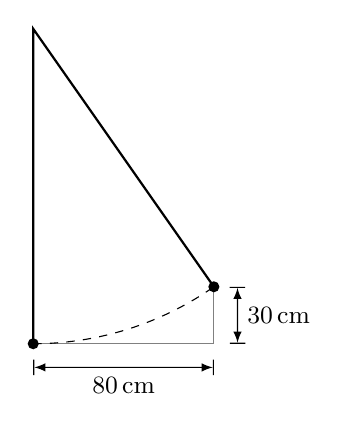
\begin{tikzpicture}[scale=1]
        % unten
        \coordinate (A) at (270:4cm);
        % oben
        \coordinate (B) at (0, 0);
        % rechts
        \coordinate (C) at (305:4cm);
        % Schnittpunkt der Hilfslinien
        \coordinate (D) at (intersection of C--[yshift=-10cm]C and A--[xshift=10cm]A);
        % Hilfslinien
        \draw[draw=white!50!black] (A) -| (C);
        % das Pendel
        \draw[line width=0.8pt] (A) -- (B) -- (C);
        % Kreislinie
        \draw[style=dashed] (A) arc (270:305:4cm);
        % Gewichte
        \fill (A) circle (2pt);
        \fill (C) circle (2pt);
        % Masse
        \draw[|<->|, >=latex] ([yshift=-3mm]A) -- node[below]{{\small80\,cm}} ([yshift=-3mm]D);
        \draw[|<->|, >=latex] ([xshift=3mm]C) -- node[right]{{\small30\,cm}} ([xshift=3mm]D);
      \end{tikzpicture}
    \end{center}
  \fi
  %\ifoutline\outline
  %\fi
  %\ifoutcome\outcome
  %\fi
\end{exercise}
